\documentclass{beamer}
\usepackage{hyperref}
\usetheme{Berlin} % Bawcie się tym do woli
\usecolortheme{seahorse} % Bawcie się tym do woli
% Większość tych package'y to rzeczy które przeklejam z jakiejś starej templatki i pewnie nie wszystkie są potrzebne
\usepackage[polish]{babel}
\usepackage[utf8]{inputenc}
\usepackage[T1]{fontenc}
\usepackage{amsmath}
\usepackage{amssymb,amsfonts,amsthm}
\usepackage{multicol}
\usepackage{array}
\usepackage{geometry}
\usepackage{listings}
\usepackage{graphicx}
\usepackage{tabularx}
\usepackage{float}
\usepackage{hyperref}
\usepackage{mathspec} % wczytuje również fontspec
\setmainfont{Latin Modern Roman}
\setromanfont{Latin Modern Roman}
\setsansfont{Latin Modern Sans}
\setmonofont{Latin Modern Mono}
\setmathrm{Latin Modern Math}
\setmathfont(Digits,Latin)[Scale=MatchLowercase]{Latin Modern Math}
% \usepackage{minted} %To chyba package do wklejania kodu

\title{Porównanie algorytmów kryptografii asymetrycznej i zastosowania}
\author{Autorzy:\\ Krzysztof Dąbrowski\\ Hussein Hazime\\ Krzysztof Rudnik\\ Piotr Szczerba\\ Jakub Więcław}
\date{2025-03-24}


\begin{document}

\begin{frame}
    \titlepage
\end{frame}

% Piotrek
\section{Wstęp}

\begin{frame}{Czym jest kryptografia asymetryczna}
    \begin{figure}
        \centering
            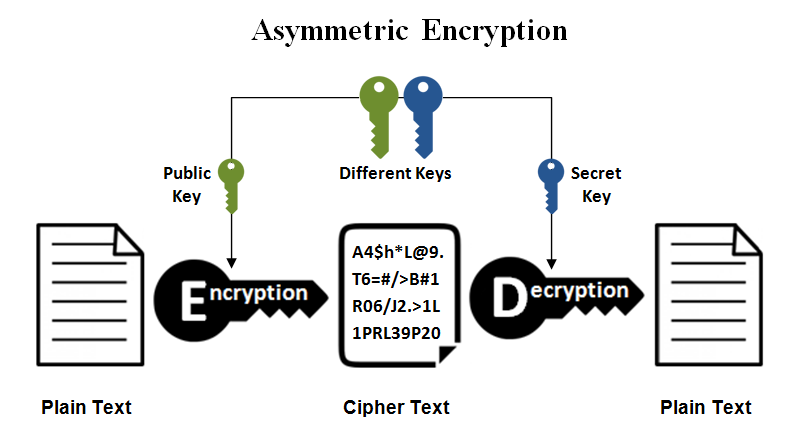
\includegraphics[height=0.45\textwidth]{introduction/graphics/Asymmetric-Encryption.png}
            \caption{Źródło: \cite{ssl2buy}}
    \end{figure}
\end{frame}

\begin{frame}{Jakie algortymy wybraliśmy}
    \begin{itemize}
        \item Puzle Merkle'a (1974)
        \item RSA (1977)
        \item ECC (1983)
    \end{itemize}

\end{frame}

\begin{frame}{Plan analizy porównawczej wybranych algorytmów}
    \begin{itemize}
        \item Podstawy matematyczne
        \pause
        \item Wykorzystanie w praktyce
        \pause
        \item Bezpieczeństwo teraz
        \pause
        \item Bezpieczeństwo w przyszłości
    \end{itemize}
\end{frame}
\section{Matematyczne podstawy algorytmów}

\begin{frame}{Puzzle Merkle'a}
    \begin{figure}
        \centering
            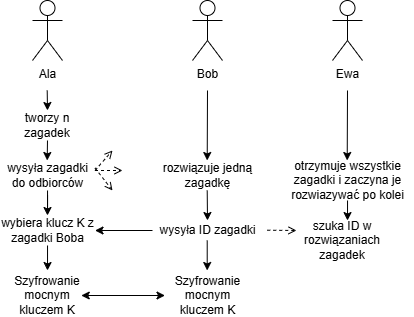
\includegraphics[height=0.45\textwidth]{teoria/graphics/ala_bob_ewa.png}
            \caption{Źródło: własne}
    \end{figure}
\end{frame}

\begin{frame}{Puzzle Merkle'a}
    \begin{center}
    \texttt{15JqVMuLIlyKdkIx} \\
    \texttt{HCzoAJ1ahv8xazFj} \\
    \texttt{9JhU04wO1o6YQ50g} \\
    \texttt{2jVyaS0JLlcKNnC9} \\
    \texttt{...} \\
    \texttt{CZ98NQLvoE9nXph6}
    \end{center}
\end{frame}

\begin{frame}{Puzzle Merkle'a}
    \begin{center}
    \texttt{15JqVMuLIlyKdkIx} \\
    \texttt{HCzoAJ1ahv8xazFj} \\
    \texttt{\textcolor{blue}{9JhU04wO1o6YQ50g}} \\ % Zmiana koloru
    \texttt{2jVyaS0JLlcKNnC9} \\
    \texttt{...} \\
    \texttt{CZ98NQLvoE9nXph6}
    \end{center}
\end{frame}

\begin{frame}{Puzzle Merkle'a}
    \begin{center}
    \texttt{\textcolor{blue}{9JhU04wO1o6YQ50g}} \\
    \pause
    $\Downarrow$ \\
    \texttt{PuzzleID: 17; NewKey: 6nph6LlaqL7YCKsY}
    \end{center}
\end{frame}

\begin{frame}{Puzzle Merkle'a}
    Trudność złamania:
    \begin{center}
        {\Large \( \frac{n \times m}{2} \)} \\[10pt]
    \end{center}
    \( n \) - liczba zagadek \\
    \( m \) - liczba obliczeń potrzebnych do złamania jednej zagadki
\end{frame}
% ---------------------
% Hussein
% Hussein


\begin{frame}{RSA}
    
    RSA (Rivest–Shamir–Adleman) to algorytm szyfrowania publicznego, który opiera się na trudności faktoryzacji dużych liczb.Matematyczna teoria RSA bazuje na następujących kluczowych elementach:

   1. Wybór dwóch dużych liczb pierwszych: \( p \) oraz \( q \).

   
    2. Obliczamy iloczyn tych liczb:
    \[
    n = p \times q
    \]
    Liczba \( n \) jest wykorzystywana zarówno w kluczu publicznym, jak i prywatnym.

    
    3. Funkcja Eulera dla \( n \) jest dana wzorem:
    \[
    \varphi(n) = (p-1)(q-1)
    \]

\end{frame}

\begin{frame}{RSA}
    Jest używana do obliczenia wykładnika prywatnego klucza.

    4. Wybieramy liczbę \( e \), która musi być liczbą względnie pierwszą względem \(\varphi(n)\) oraz spełnia warunek:
    \[
    \gcd(e, \varphi(n)) = 1, \quad e < \varphi(n)
    \]
    GCD: Obliczanie największego wspólnego dzielnika (GCD, greatest common divisor), oraz jest obliczany za pomocą algorytmu Euklidesa.

   
    Algorytm Euklidesa polega na powtarzaniu operacji dzielenia z resztą, aż reszta wyniesie 0.
\end{frame}

\begin{frame}{RSA}




    \begin{enumerate}
        \item Dla dwóch liczb \( a \) i \( b \), gdzie \( a \geq b \), obliczamy:
        \[
        a \div b = q \quad \text{(część całkowita)}
        \]
        \[
        r = a \mod b \quad \text{(reszta)}
        \]
        co zapisujemy jako:
        \[
        a = b \times q + r
        \]

        \item Następnie ustawiamy:
        \[
        a = b, \quad b = r
        \]
        i powtarzamy krok 1.

        \item Proces powtarzamy, aż \( b = 0 \). Gdy \( b = 0 \), wówczas:
        \[
        \gcd(a, b) = a
        \]
    \end{enumerate}



\end{frame}

\begin{frame}{RSA}
   
    5. Liczba \( d \) jest odwrotnością modularną \( e \) względem \( \varphi(n) \), tzn.:
    \[
    e \times d \equiv 1 \pmod{\varphi(n)}
    \]
   
    Należy znaleźć "modularną odwrotność" \( e \) modulo \( \varphi(n) \).

    
    W celu wyznaczenia wartości \( d \) często stosuje się \textbf{rozszerzony algorytm Euklidesa}, który nie tylko oblicza największy wspólny dzielnik (\(\gcd\)), ale również pozwala znaleźć współczynniki spełniające:

    
         \[
        e \times d + \varphi(n) \times k = \gcd(e, \varphi(n))
   \]
       
\end{frame}

\begin{frame}{RSA}
   


   
    \subsection{Klucz publiczny i prywatny}
    \begin{itemize}
        \item Klucz publiczny: \( (e, n) \)
        \item Klucz prywatny: \( (d, n) \)
    \end{itemize}

    
    6. Jeśli wiadomość \( M \) (gdzie \( M < n \)) ma zostać zaszyfrowana, obliczamy:
    \[
    C = M^e \mod n
    \]
    gdzie \( C \) to zaszyfrowana wiadomość.

   
    7. Odbiorca używa klucza prywatnego \( d \) i oblicza:
    \[
    M = C^d \mod n
    \]
\end{frame}


\begin{frame}{ECC}


Kryptografia krzywych eliptycznych (ECC) jest definiowana za pomocą następującego ogólnego równania w dwóch zmiennych z współczynnikami:

\[
    y^2 = x^3 + ax + b
\]

gdzie $a$ i $b$ są współczynnikami krzywej eliptycznej.

Delta krzywej eliptycznej jest określony jako:

\[
    \Delta = 4a^3 + 27b^2 \neq 0
\]

Warunek $\Delta \neq 0$ zapewnia, że krzywa tworzy \textbf{grupę algebraiczną}, co jest konieczne do zastosowania jej w kryptografii. Jeśli $\Delta = 0$, struktura matematyczna krzywej nie jest prawidłowa do użycia w szyfrowaniu.
\end{frame}

\begin{frame}{ECC}

    \textbf{Globalne elementy publiczne:}
    \begin{itemize}
        \item Wybór krzywej eliptycznej $E_q(a, b)$
        \item Wybór punktu bazowego $G(x, y)$ o dużym rzędzie $n$.
    \end{itemize}

    \textbf{Generowanie klucza Użytkownika A:}
    \begin{itemize}
        \item Użytkownik A wybiera klucz prywatny $V_A$, gdzie $V_A < n$.
        \item Oblicza klucz publiczny $P_A(x, y) = V_A \times G(x, y)$.
    \end{itemize}

    \textbf{Generowanie klucza Użytkownik B:}
    \begin{itemize}
        \item Użytkownik B wybiera klucz prywatny $V_B$, gdzie $V_B < n$.
        \item Oblicza klucz publiczny $P_B(x, y) = V_B \times G(x, y)$.
    \end{itemize}

\end{frame}


\begin{frame}{ECC}

    \begin{itemize}
        \item Użytkownik A wybiera wiadomość $P_m(x, y)$ oraz losową liczbę $k$, gdzie $1 < k < q$.
        \item Tworzy szyfrogram $C_m = ((k \times G(x, y)), (P_m(x, y) + k \times P_B(x, y)))$.
    \end{itemize}
    \begin{itemize}
        \item Użytkownik B otrzymuje szyfrogram $C_m$ jako $((x, y), (x', y'))$.
        \item Odszyfrowuje wiadomość:
        \[
            P_m(x, y) = (P_m(x, y) + k \times P_B(x, y)) - (k \times V_B \times G(x, y))
        \]
        \item Po wykonaniu operacji pozostaje oryginalna wiadomość $P_m(x, y)$.
    \end{itemize}


\end{frame}


% ---------------------
% KUBA

% Od tego momentu porównujemy algorytmy między sobą
\section{Zastosowania}

\subsection{Uwierzytelnianie}
\begin{frame}{Uwierzytelnianie}
    \begin{itemize}
        \pause
        \item Podpisy cyfrowe
        \pause
        \item Certifikaty
    \end{itemize}
\end{frame}

\begin{frame}{Podpisy cyfrowe - charakterystyka}
\pause
    \begin{itemize}
        \item Uwierzytelnianie nadawcy
        \pause
        \item Integralność danych
        \pause
        \item Niezaprzeczalność
    \end{itemize}
    
\end{frame}

\begin{frame}{Podpisy cyfrowe - metoda działania}
    \begin{columns}
        \column{0.5\textwidth}
        \textbf{RSA}
        \begin{itemize}
            \item Hashowanie wiadomości
            \item Szyfrowanie hashu kluczem prywatnym
            \item Odszyfrowanie hashu kluczem publicznym
            \item Porównanie hashy
        \end{itemize}

        \column{0.5\textwidth}
        \textbf{ECC (ECDSA)}
        \begin{itemize}
            \item Hashowanie wiadomości
            \item Generowanie losowej wartości $k$
            \item Obliczenie $(r, s)$
            \item Porównanie podpisu
        \end{itemize}
        \vspace{6pt}
    \end{columns}
\end{frame}

\begin{frame}{Certifikaty - budowa}
    \begin{itemize}
        \item Dane o właścicielu
        \item Klucz publiczny
        \item Podpis cyfrowy
        \item Okres ważności
        \item Algorytm podpisu
    \end{itemize}

\end{frame}

\begin{frame}{Certifikaty - działanie}
    \begin{itemize}
        \item Wysłanie certyfikatu do serwera
        \item Serwer sprawdza ważność i poprawność certyfikatu
        \item Po pozytywnej weryfikacji serwer szyfruje sesję i kontynuuje komunikację
    \end{itemize}
    
\end{frame}

\begin{frame}{Certyfikaty - algorytmy}

    \begin{columns}
        \column{0.5\textwidth}
        \centering
        
        \textbf{RSA}
        \begin{itemize}
            \item Powszechnie stosowany historycznie
            \item Większe klucze $\rightarrow$ większe wymagania sprzętowe
        \end{itemize}
        
        \column{0.5\textwidth}
        \centering

        \textbf{ECC}  
        \begin{itemize}
            \item Coraz popularniejszy
            \item Krótsze klucze $\rightarrow$ mniejsze wymagania sprzętowe
        \end{itemize}
        \vspace{7.5pt}

    \end{columns}

\end{frame}


\subsection{}
\begin{frame}{Kryptowaluty}
    \begin{center}
        \begin{minipage}{0.24\textwidth}
            \centering
            
\includegraphics[width=\linewidth]{applications/graphics/Bitcoin.png} \\
            \tiny{Źródło: \href{https://commons.wikimedia.org/wiki/File:Bitcoin_logo.svg}{commons.wikimedia.org}}
        \end{minipage}
        \hfill
        \begin{minipage}{0.24\textwidth}
            \centering
            
\includegraphics[width=\linewidth]{applications/graphics/Ethereum.png} \\
            \tiny{Źródło: \href{https://camo.githubusercontent.com/1b3d0063d6a8bcd56ca07b0ea2ef0f71b17a0fa8/687474703a2f2f737667706f726e2e636f6d2f6c6f676f732f657468657265756d2e737667}{camo.githubusercontent.com}}
        \end{minipage}
        \hfill
        \begin{minipage}{0.24\textwidth}
            \centering
            
\includegraphics[width=\linewidth]{applications/graphics/Dogecoin.png} \\
            \tiny{Źródło: \href{https://altcoinsbox.com/dogecoin-logo/}{altcoinsbox.com}}
        \end{minipage}
        \hfill
        \begin{minipage}{0.24\textwidth}
            \centering
            
\includegraphics[width=\linewidth]{applications/graphics/Litecoin.jpg} \\
            \tiny{Źródło: \href{https://cryptologos.cc/litecoin}{cryptologos.cc}}
        \end{minipage}
    \end{center}
\end{frame}



\begin{frame}{Komunikatory E2E - metoda działania}
    \begin{itemize}
        \item Wiadomości są widoczne tylko dla nadawcy i odbiorcy
        \item Klucz publiczny jest przesyłany do serwera
        \item Serwer przesyła klucz publiczny do odbiorcy
        \item Odbiorca odszyfrowuje wiadomość kluczem prywatnym
    \end{itemize}
\end{frame}
\begin{frame}{Komunikatory E2E - przykłady}
    \begin{center}
        \begin{minipage}{0.1\textwidth}
            
\includegraphics[width=\textwidth]{applications/graphics/Signal.png}
        \end{minipage}
        \begin{minipage}{0.6\textwidth}
            \textbf{X3DH oraz Curve25519}
        \end{minipage}

        \vspace{0.3cm}

        \begin{minipage}{0.1\textwidth}
            
\includegraphics[width=\textwidth]{applications/graphics/WhatsApp.png}
        \end{minipage}
        \begin{minipage}{0.6\textwidth}
            \textbf{Curve25519}
        \end{minipage}

        \vspace{0.3cm}

        \begin{minipage}{0.1\textwidth}
            
\includegraphics[width=\textwidth]{applications/graphics/Messenger.png}
        \end{minipage}
        \begin{minipage}{0.6\textwidth}
            \textbf{Signal Protocol}
        \end{minipage}

        \vspace{0.3cm}

        \begin{minipage}{0.1\textwidth}
            
\includegraphics[width=\textwidth]{applications/graphics/Imessage.png}
        \end{minipage}
        \begin{minipage}{0.6\textwidth}
            \textbf{RSA-2048 oraz ECDSA/ECDH}
        \end{minipage}
    \end{center}
\end{frame}

\begin{frame}{IoT}
    \begin{itemize}
        \item Uwierzytelnianie urządzeń (RSA/ECC)
        \item Szyfrowanie komunikacji (TLS, MQTT-TLS)
        \item Bezpieczne aktualizacje OTA
    \end{itemize}
\end{frame}

% ---------------------
% Krzysiek D
\section{Bezpieczeństwo}
% Porównanie bezpieczeństwa algorytmów RSA i ECC w zastosowaniu na aktualnymi technologiami

% Jak porównywać bezpieczeństwo algorytmów
\begin{frame}{Porównywanie bezpieczeństwa}
\textbf{Bity bezpieczeństwa \cite{BitSecurityOfCryptographicPrimitives}}
\pause
\begin{itemize}
    \pause
    \item Pojedyncza liczba
    \pause
    \item \( x = \log_2(N) \)
    \item \( x \) - liczba bitów bezpieczeństwa
    \item \( N \) - średnia ilość operacji wymaganych do złamania szyfru
\end{itemize}
\pause
\vspace{8mm}

\textit{Algorytm o sile 20 bitów bezpieczeństwa wymaga średnio $2^{20} = 1048576$ operacji do złamania.}

\end{frame}

\begin{frame}{Bezpieczeństwo RSA}
% Wielkość klucza to ilość bitów modułu n = p*q
Najszybszy klasyczny \footnote{tz. nie korzystający z matematyki kwantowej} algorytm refaktoryzacji liczb to Ogólne sito ciała liczbowego (GNFS) \footnote{ang. General Number Field Sieve}.
\pause
\begin{itemize}
    \item Złożoność \cite{GNFSImplementation} \begin{footnotesize}$$L(n) = \exp\left(\left(\frac{64}{9}\right)^{1/3} (\ln n)^{1/3} (\ln \ln n)^{2/3}\right)$$\end{footnotesize}
    \pause
    \item Liczba bitów bezpieczeństwa $= \log_2(L(n))$
\end{itemize}
\pause
$$
\begin{array}{|c|c|}
\hline
\textbf{Wielkość \, klucza \, RSA \, (bity)} & \textbf{Bity \, Bezpieczeństwa} \\
\hline
1024 & \sim 80 \\
2048 & \sim 112 \\
3072 & \sim 128 \\
\hline
\end{array}
$$
\end{frame}

\begin{frame}{Bezpieczeństwo ECC}
% Wielkość klucza to rozmiar jednego wymiaru dyskretnej przestrzeni
Najszybszy klasyczny \footnote{tz. nie korzystający z matematyki kwantowej} algorytm do rozwiązania ECDLP to algorytm faktoryzacji rho Pollarda \cite{SolvingECDLP}.
\pause
\begin{itemize}
    \item Dla przestrzeni wielkości k wymaga $\sqrt{k}$ kroków
    \item Do x bitów bezpieczeństwa potrzebny jest klucz wielkości 2x
    \pause
    \item Przykładowo 256-bitowa krzywa teoretycznie daje 128-bitów bezpieczeństwa
\end{itemize}
\pause
Rzeczywiste bezpieczeństwo $\approx 0.886*\sqrt{k}$
\pause
\begin{itemize}
    \item \textit{secp256k1} klucz 256 bit $\Rightarrow$ 127.8 bitów bezpieczeństwa \cite{Secp256k1Security}
    \item \textit{Curve448} klucz 448 bit $\Rightarrow$ 222.8 bitów bezpieczeństwa \cite{Secp256k1Security}
\end{itemize}
% Rzeczywiste bezpieczeństwo jest mniejsze, ponieważ ranga krzywej w dyskretnej przestrzeni jest zazwyczaj mniejsza niż wielkość pojedynczego wymiaru przestrzeni

\end{frame}

\begin{frame}{Porówanie długości klucza}
    \begin{figure}
        \centering
            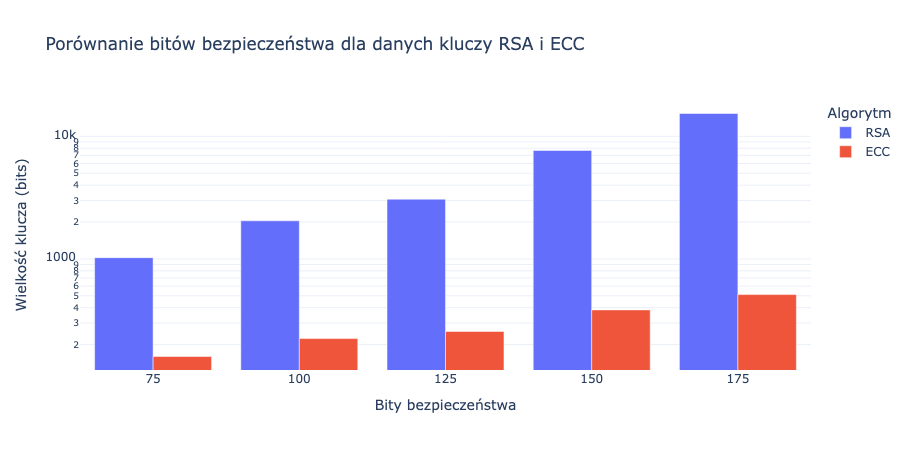
\includegraphics[width=\textwidth]{security/graphics/Porównanie bitów bezpieczeństwa dla danych kluczy RSA i ECC}
            \caption{Porównanie bitów bezpieczeństwa dla danych kluczy RSA i ECC}
    \end{figure}
\end{frame}

\begin{frame}{Podatności ECC}
\framesubtitle{Podatne implementacje}
\textbf{$ECDLP \neq ECC$} \\
\pause
Bezpieczne implementacje są teoretycznie możliwe. \\
\pause
Implementacja może być podatna na \cite{SafeCurves}
\begin{itemize}
    \item Ataki na generator liczb losowych
    \item Błędne wyniki dla specyficznych punktów
    \item Wyciek informacji, gdy podany punkt nie należy do krzywej
    \item Ataki poprzez pomiar czasu wykonania
\end{itemize}
\pause
\vspace{3mm}
Przykład: Wyciek kluczy prywatnych Sony PlayStation 3 w 2010 \cite{ConsoleHacking2010}
% W 2010 roku odkryto, że implementacja ECDSA w PlayStation 3 miała poważny błąd.
% Błąd polegał na używaniu tej samej wartości nonce dla różnych podpisów.
% Pozwoliło to na odzyskanie klucza prywatnego z dwóch podpisów cyfrowych.
% W wyniku tego ataku możliwe było uruchamianie nieautoryzowanego oprogramowania na konsoli.
\end{frame}

\begin{frame}{Podatności ECC}
\framesubtitle{Podatne krzywe}
Nie wszystkie krzywe gwarantują, że ECDLP jest trudny.
Ataki na podatne krzywe \cite{WeakCurvesInEllipticCurveCryptography}
\begin{itemize}
    \item Algorytm Pohinga-Hellmana
    \item Algorytm Smarta
\end{itemize}
\pause
\vspace{3mm}
Możliwe jest \textbf{celowe wybranie słabej krzywej} jako backdoor.
\end{frame}

\begin{frame}{Podatności ECC}
    \framesubtitle{Bezpieczny system}
    Standardy wyboru krzywych \cite{SafeCurves}
    \begin{scriptsize}
        \begin{itemize}
            \item ANSI X9.62 (1999)
            \item IEEE P1363 (2000)
            \item SEC 2 (2000)
            \item NIST FIPS 186-2 (2000)
            \item ANSI X9.63 (2001)
            \item Brainpool (2005)
            \item NSA Suite B (2005)
            \item ANSSI FRP256V1 (2011)
        \end{itemize}
    \end{scriptsize}
    \pause
    \vspace{3mm}
    Wśród przebadanych krzywych są też bardziej wydajne krzywej z mniejszym bezpieczeństwem dla tej samej długości klucza. \cite{PracticalCryptographyForDevelopers}
\end{frame}

\begin{frame}{Ataki na RSA}
\begin{itemize}
    \item Ataki kanału bocznego
    \item Ataki na generator liczb losowych
    \pause
    \item \textbf{Podatne liczby pierwsze}
    \pause
    \item \textbf{Długość klucza}
\end{itemize}
Klucze długości 1024 bit są dziś niewystarczająco bezpieczne.
\end{frame}

\begin{frame}{Użycie bibliotek}
\pause
\begin{figure}
    \centering
        
\includegraphics[height=0.55\textwidth]{security/graphics/developer-implements-rsa-car-meme}
        \caption{Źródło: \cite{SeriouslyStopUsingRsa}}
\end{figure}
\end{frame}

% ---------------------
% Krzysiek R
\section{Przyszłość}
\begin{frame}{Przyszłość w kontekście komputerów kwantowych}
       Algorytm Shore'a:
        \begin{itemize}
            \item Kwantowy algorytm rozkładu na czynniki
            \item Działa w czasie wielomianowym dla problemów faktoryzacji i logarytmu dyskretnego.
            \item Stosowany do RSA: rozkład liczby $N$ na czynniki pierwsze.
            \item Stosowany do ECC: rozwiązanie problemu logarytmu dyskretnego na krzywych eliptycznych.
        \end{itemize}
\end{frame}
\begin{frame}{Porównanie wymagań kwantowych}
    \begin{itemize}
        \item Liczba kubitów i operacji Toffoli dla RSA i ECC: \cite{quantum}
        \begin{itemize}
            \item RSA-3072 wymaga 6146 kubitów i $1.86 \times 10^{13}$ operacji Toffoli.
            \item ECC-P256 wymaga 2330 kubitów i $1.26 \times 10^{11}$ operacji Toffoli.
        \end{itemize}
        \item ECC wymaga mniej zasobów kwantowych niż RSA o równoważnym poziomie bezpieczeństwa.
    \end{itemize}
\end{frame}
\begin{frame}{Implikacje dla bezpieczeństwa}
    \begin{itemize}
        \item Komputery kwantowe będą mogły szybciej złamać ECC niż RSA.
        \item NIST(National Institute of Standards and Technology) pracuje nad postkwantową kryptografią (np. schematy oparte na kratkach).
        \item Organizacje powinny rozważyć migrację do algorytmów odpornych na komputery kwantowe.
    \end{itemize}
\end{frame}
\begin{frame}
    \frametitle{Dlaczego ECC jest bardziej podatne?}
    \begin{itemize}
        \item ECC bazuje na krótszych kluczach niż RSA (przy tej samej odporności klasycznej)
        \item ECC 256-bit odpowiada RSA 3072-bit pod względem klasycznej odporności.
        \item Shor’s Algorithm atakuje bezpośrednio strukturę matematyczną – mniejsze klucze ECC oznaczają, że wymagana liczba kubitów do ataku jest mniejsza
        \item W praktyce, ECC może zostać złamane szybciej niż RSA na komputerze kwantowym
    \end{itemize}
\end{frame}






% \begin{frame}{Bell's Theorem} % Opcjolanlne

% \end{frame}

% \begin{frame}{Regulacje prawne}
% \end{frame}
\begin{frame}{Regulacje prawne}
    \begin{itemize}
            \item Przepisy dotyczące szyfrowania różnią się w zależności od kraju.
            \item Kraje o restrykcyjnych przepisach, np. Chiny, mogą wymagać krajowych algorytmów.
            \item Wyzwania związane z międzynarodową zgodnością i polityką ochrony danych.
            \item Organizacje muszą dostosować swoje procedury do różnych regulacji.
    \end{itemize}
\end{frame}
\begin{frame}{Bezpieczeństwo a prywatność}
    \begin{itemize}
        \item Zrównoważenie ochrony prywatności z potrzebami organów ścigania.
        \item Wprowadzenie przepisów o backdoorach w systemach szyfrowania.
        \item Przepisy umożliwiające dostęp do zaszyfrowanych danych przez służby.
        \item Ryzyko naruszenia prywatności w imię bezpieczeństwa narodowego.
    \end{itemize}
\end{frame}
\begin{frame}{Przyszłość kryptografii w kontekście komputerów kwantowych}
    \begin{itemize}
    \item RSA i ECC może zostać złamane przez komputery kwantowe.
    \item Wymóg przejścia na post-kwantowe algorytmy szyfrowania.
    \item Nowe algorytmy, takie jak lattice-based cryptography, mogą stać się standardem.
    \item Regulacje mogą wymagać implementacji algorytmów odpornych na ataki kwantowe.
    \end{itemize}
\end{frame}
\begin{frame}{Podsumowanie}
    \begin{itemize}
        \item Komputery kwantowe mogą zagrażać bezpieczeństwu RSA i ECC.
        \item NIST pracuje nad algorytmami odpornymi na ataki kwantowe.
        \item Organizacje muszą dostosować swoje procedury do nowych wyzwań.
        \item Bezpieczeństwo i prywatność muszą być zrównoważone w regulacjach.
    \end{itemize}
\end{frame}

% \section{Przyszłość}
% \begin{frame}{ECC jest łatwiejsze do złamania przez algorytm Shore'a niż RSA}

% \end{frame}
% \begin{frame}{Bell's Theorem} % Opcjolanlne

% \end{frame}

% \begin{frame}{Regulacje prawne}

% \end{frame}
% ---------------------
\begin{frame}[allowframebreaks, noframenumbering]{Bibliografia}
\printbibliography
\end{frame}

\end{document}
